% !TeX spellcheck = en_US
\subsection{Log encoding}
This encoding utilize the fact that each propositional variable can only take one of two values, i.e. either True or False.

\subsubsection{Encoding the variables}
First we encode each possible value from the domain with a distinct binary representation. Depending on the maximum number of bits needed to encoded all the domain values, an equal number of propositional variables for each CSP variable is generated. So if the size of domain was $m$ and the number of CSP variables was $n$, we need $n \lceil \log_2 m \rceil$ propositional variable on the SAT side.

Notice that encoding each value from the CSP variable's domain means that the size of this domain must be exactly equal to $2^i$, which is not necessary the case. So extra possible binary representations can emerge (implied in the formula by the ceiling function, i.e. if $ \lceil \log_2 m \rceil > \log_2 m $). To avoid assigning these invalid values to any CSP variable we have to include extra clauses to ensure that a variable can't be assigned a value outside its domain. 

On the other hand, unlike the direct encoding we do not need any additional clauses to ensure that each CSP variable is given a value at all (ALO clauses) nor to ensure that each CSP variable is given only one value (AMO clauses).

The same example from above is used to demonstrate the additional needed clauses. The CSP constraints are not listed explicitly but rather illustrated by the borders on the map.

\begin{figure}[H]
	\centering
	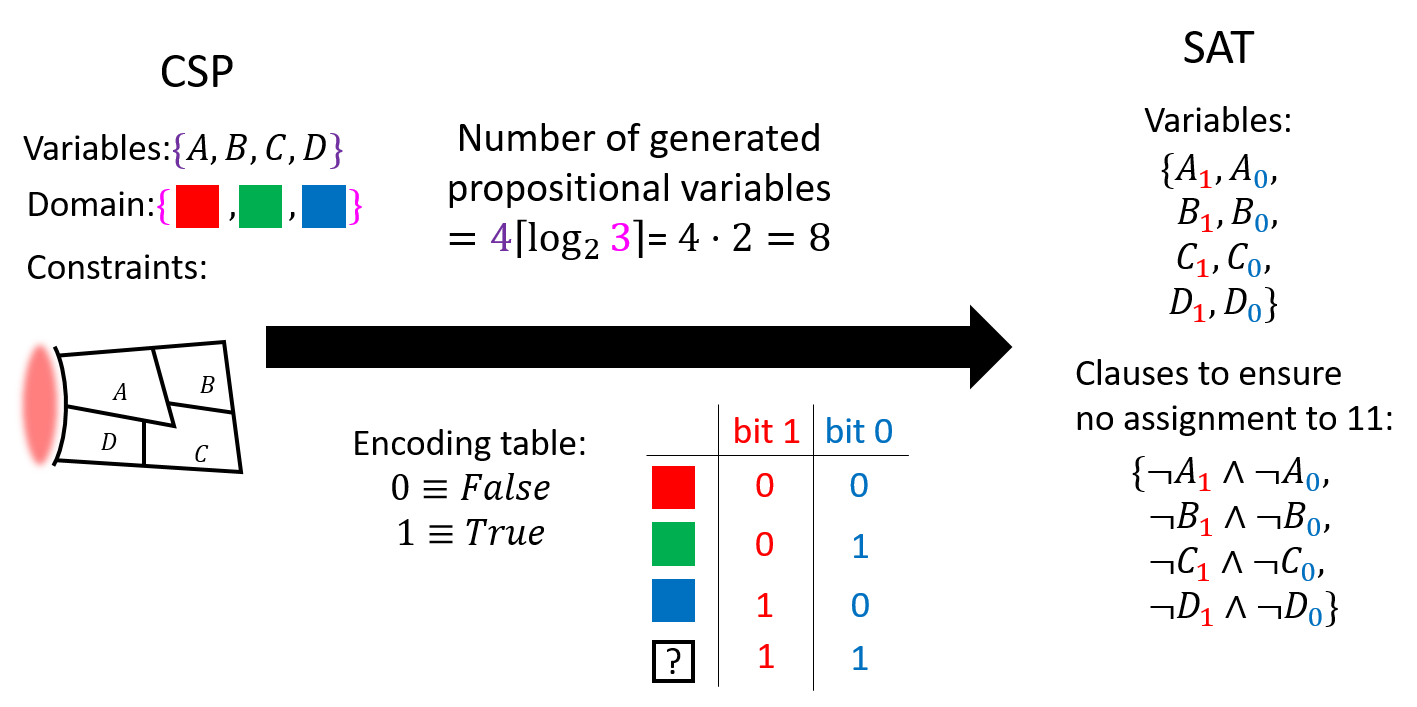
\includegraphics[width=0.85\linewidth]{assets/log_variables}
	\captionsetup{justification=centering,margin=2cm}
	\caption{Encoding CSP variables using log encoding}
	\label{fig:log_variables}
\end{figure}

Notice that the log encoding generates less propositional variables than direct encoding. Anyway, this fact does not improve the performance of DPLL on the generated SAT instance because more steps are required to untangle the problem as discussed later. \ref{subsec:log_proposition}

\subsubsection{Encoding the constraints}
As discussed before, constraints could be unary, binary or n-ary. Since any n-ary constraint can be expanded to multiple binary constraints, the main focus will be on encoding only the unary and the binary constraints.

Encoding unary constraints is straight forward. For example to ensure that a CSP variable $X$ can't be assigned a certain value from its domain encoded in the binary form $01$, we only need to add the following clause to the SAT formula: $\neg (\neg X_1 \wedge X_0) \equiv X_1 \vee \neg X_0$. Remember that the subscript of the propositional variables $X_0, X_1$ corresponds to the position of the bit in the binary form of the CSP value.

Encoding binary constraints can be done in similar manner. For example to encode the CSP constraint $A \neq D$, where $A$ and $D$ can be either green \textcolor{green}{$\blacksquare$} or blue \textcolor{blue}{$\blacksquare$} (i.e. their domain is $\{ \textcolor{green}{\blacksquare}, \textcolor{blue}{\blacksquare} \}$) with the binary representations \textcolor{green}{$01$} and \textcolor{blue}{$10$} respectively, we need to include the following clauses in our SAT:
\begin{figure}[H]
	\centering
	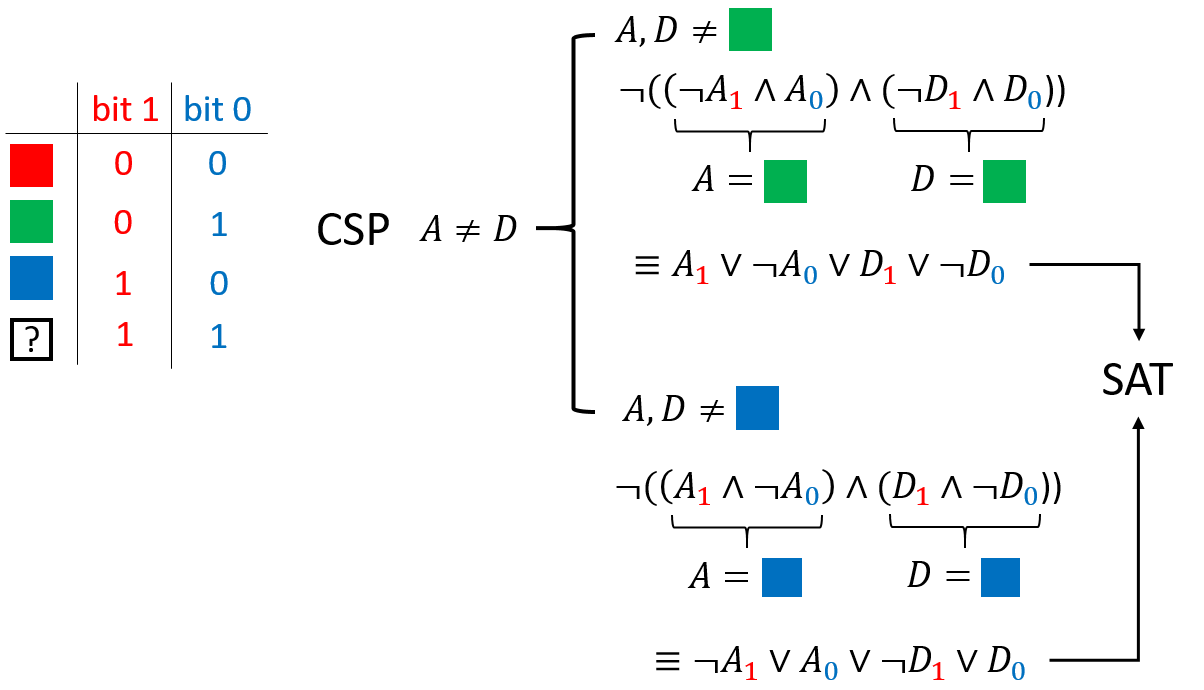
\includegraphics[width=0.7\linewidth]{assets/binary_constraints_log_encoding}
	\captionsetup{justification=centering,margin=2cm}
	\caption{Encoding binary CSP constraint using log encoding}
	\label{fig:binary_constraints_log_encoding}
\end{figure}

\subsubsection{Proposition}\label{subsec:log_proposition}
In spite of the fact that log encoding generate fewer variables on the SAT side than direct encoding, it is easy to see that DPLL applied on log encoded CSP is dominated by FC applied to the original CSP problem (assuming equivalent branching heuristics).

\subsubsection{Proof idea}
The proof idea is similar to the proof mentioned earlier for the direct encoding case \ref{subsec:direct_encoding_proof}. We process by comparing the search trees of each algorithm. First we show that both trees must have at least equal number of branches. By Induction on each CSP variable $X$, FC algorithm will branch upon it. On the SAT side DPLL will consider all propositional variables corresponding to the same CSP variable ($X_i \dots X_{\lceil \log_2 m \rceil}$), where $m$ is the size of the domain.

Further more, we can exploit the natural logarithmic behavior of log encoding on the search tree to show that DPLL is \textbf{strictly} dominated by FC. This can be done using a simple example. Consider a CSP consists of two variables $A$ and $B$ with domain of size 3 and no constraints other than rolling out all assignments. FC will require three branches for each variable to show that this problem is unsatisfiable. Since the size of the domain equals 3, we need at least two bits to represent each CSP variable. Therefore, DPLL must branch at least $2 * 2 * 2 = 8$ times to show that the problem is unsatisfiable (the first 2 represents for the number of variables, the second one for the number of bits, and the last one to indicate branching on each case True or False as discussed before).

\begin{figure}[H]
	\centering
	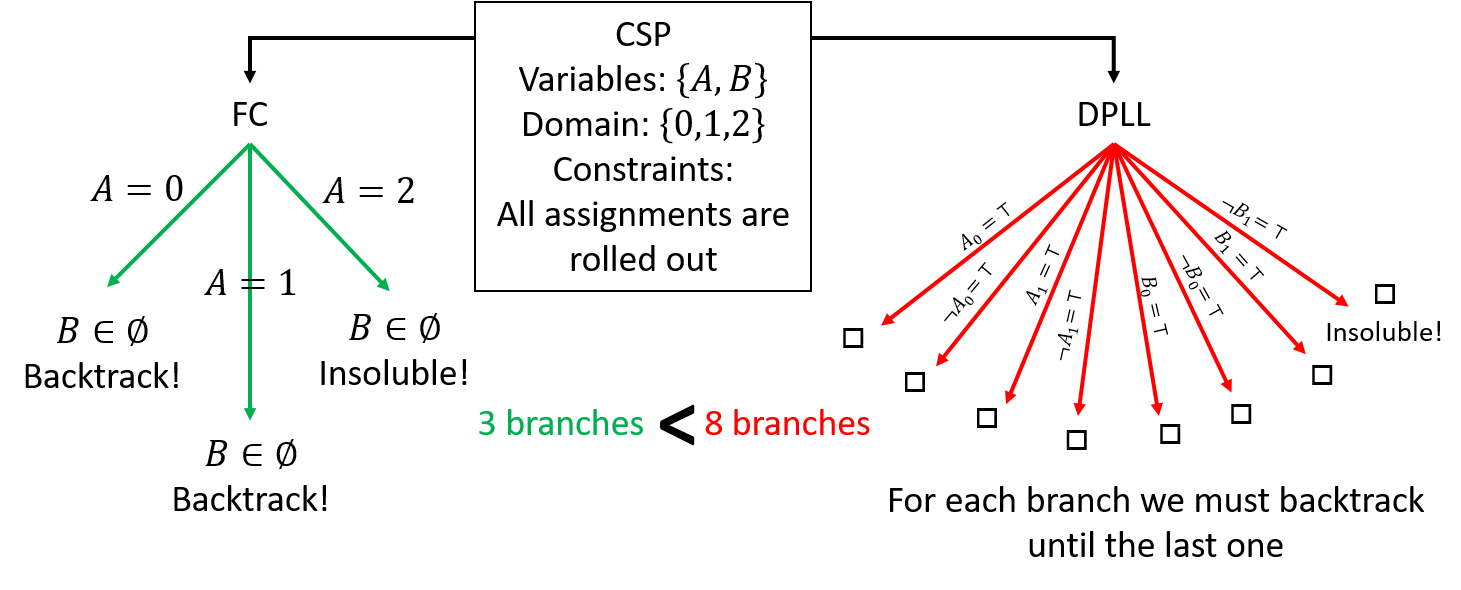
\includegraphics[width=0.85\linewidth]{assets/log_dominated_by_fc}
	\captionsetup{justification=centering,margin=2cm}
	\caption{Seach trees of DPLL and FC for trivial CSP}
	\label{fig:log_dominated_by_fc}
\end{figure}



